\chapter{Wybrane metody fuzji sygnałów}
\label{chap:wybrane}

Z racji tego, że każdy z omówionych czujników ruchu posiada swoje niedoskonałości, takie jak dryf kątów obrotu obliczonych na podstawie odczytów z żyroskopu, brak odporności na szybkozmienne zakłócenia akcelerometru oraz wpływ ferromagnetyków na odczyty magnetometru, konieczna jest fuzja pochodzących z czujników sygnałów, za pomocą dostępnych algorytmów, w celu osiągnięcia zadowalającego rezultatu obliczonych rotacji wokół osi. Za zadowalający rezultat, uznaje się brak dryfu, brak zakłóceń szybkozmiennych oraz skompensowane stałe zakłócenia pochodzące z ferromagnetyków w pobliżu czujnika. W tym celu zaimplementowano i przetestowano trzy znane algorytmy wykorzystywane w zakresie fuzji sygnałów:
\begin{itemize}
    \item Filtr komplementarny
    \item Filtr Kalmana
    \item Filtr Madgwicka
\end{itemize}

%----------------------------------------------------------------------------------------------------------------
\section{Filtr komplementarny}

Jednym z łatwiejszych w implementacji filtrów używanych do fuzji dwóch lub większej ilości sygnałów, jest filtr komplementarny. Zasada działania tego filtra opiera się o filtr dolno i górno przepustowy, za pomocą których eliminujemy zakłócenia wolno i szybko zmienne. Przedstawiony poniżej algorytm filtra komplementarnego opracowano w oparciu o artykuł \cite{Komplementarny2}. Schemat filtra znajduje się na rysunku \ref{filtr komplementarny}

\begin{figure}[h!]
    \centering
    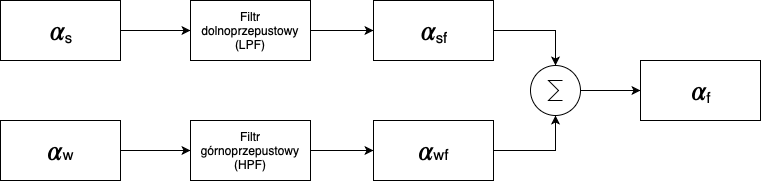
\includegraphics[width=0.75\textwidth]{Rysunki/Rozdzial04/Filtr_komplementarny.png}
    \caption{Schemat blokowy filtra komplementarnego}
    \label{filtr komplementarny}
\end{figure}

dla którego

$\alpha_s$ -- pomiar kąta obarczony szybko-zmiennymi zakłóceniami

$\alpha_{sf}$ -- pomiar kąta pozbawiony szybko-zmiennych zakłóceń

$\alpha_w$ -- pomiar kąta obarczony wolno-zmiennymi zakłóceniami

$\alpha_{wf}$ -- pomiar kąta pozbawiony wolno-zmiennych zakłóceń

$\alpha_f$ -- kąt po odfiltrowaniu zakłóceń

%----------------------------------------------------------------------------------------------------------------
\subsection{Filtr dolnoprzepustowy}

Za pomocą filtra dolnoprzepustowego eliminujemy zakłócenia szybko zmienne (charakterystyczne, np. dla akcelerometru lub magnetometru) powyżej częstotliwości granicznej, która powiązana jest ze stałą czasową w następujący sposób
$$
    f_{gr} = \frac{1}{2\pi RC} = \frac{1}{2\pi\tau}
$$

Dyskretny wzór na sygnał wyjściowy z filtra dolnoprzepustowego, można wyprowadzić w oparciu o model obwodu RC, w którym iloczyn wartości R i C stanowi wartość stałej czasowej filtra $\tau$.

\begin{figure}[htb!]
    \centering
    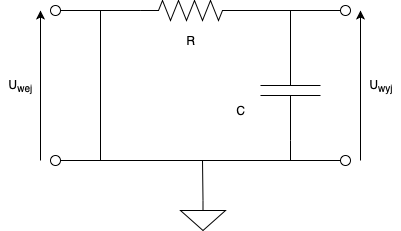
\includegraphics[width=0.5\textwidth]{Rysunki/Rozdzial04/FIltr_dolnoprzepustowy.png}
    \caption{Filtr dolnoprzepustowy RC}
    \label{filtr dp}
\end{figure}

Transmitancja filtra dolnoprzepustowego
$$
    \frac{U_{wyj}}{U_{wej}} = \frac{1}{RCs + 1} = \frac{1}{\tau s + 1}
$$
Na podstawie transmitancji otrzymujemy wzór na wartość napięcia wejściowego filtra
$$
     U_{wej} = RC\Dot{U}_{wyj} + U_{wyj} = \tau \Dot{U}_{wyj} + U_{wyj}
$$
Następnie wprowadzając oznaczenia $x = U_{wej}$ oraz $y = U_{wyj}$ i przekształcając wzór względem wartości wyjściowej $y$ otrzymujemy wzór na dyskretną wartość na wyjściu filtra 
\begin{equation}
    y(t) = x(t)\frac{\Delta t}{\tau + \Delta t} + y(t-1)\frac{\tau}{\tau + \Delta t} = \gamma x(t) + (1 - \gamma)y(t-1)
    \label{wyjscie dp}
\end{equation}
dla którego
$$
    0 \leq \gamma \leq 1,
    \quad
    \tau = \Delta t\left(\frac{1 - \gamma}{\gamma}\right)
$$

%----------------------------------------------------------------------------------------------------------------
\subsection{Filtr górnoprzepustowy}

Jeśli mamy do czynienia z zakłóceniami wolno zmiennymi (np. w przypadku żyroskopu) korzysta się z filtra górnoprzepustowego, odcinającego zakłócenia poniżej częstotliwości granicznej, która związana jest ze stałą czasową w taki sam sposób, jak w przypadku filtra dolnoprzepustowego.
$$
$$

\begin{figure}[htb!]
    \centering
    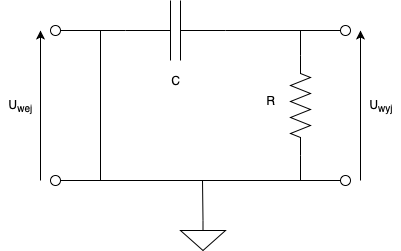
\includegraphics[width=0.5\textwidth]{Rysunki/Rozdzial04/FIltr_gornoprzepustowy.png}
    \caption{Filtr górnoprzepustowy CR}
    \label{filtr gp}
\end{figure}

Transmitancja filtra górnoprzepustowego
$$
    \frac{U_{wyj}}{U_{wej}} = \frac{RCs}{RCs + 1} = \frac{\tau s}{\tau s + 1}
$$
Postępując analogicznie jak w przypadku filtra dolnoprzepustowego otrzymujemy zależności pomiędzy napięciem wejściowym, a wyjściowym
$$
   RC\Dot{U}_{wyj} + U_{wyj} = RC\Dot{U}_{wej} \Rightarrow \tau\Dot{U}_{wyj} + U_{wyj} = \tau\Dot{U}_{wej} 
$$
Wprowadzając oznaczenia, jak w przypadku filtra dolnoprzepustowego otrzymujemy wzór na dyskretną wartość wyjściową
\begin{equation}
    y(t) = \tau\frac{x(t) - x(t-1)}{\Delta t} - \frac{y(t) - y(t-1)}{\Delta t}  = \beta y(t-1) + \beta(x(t) - x(t-1))
    \label{wyjscie gp}
\end{equation}
dla której
$$
    0 \leq \beta \leq 1,
    \quad
    \tau = \Delta t\left(\frac{\beta}{1 - \beta}\right)
$$

%----------------------------------------------------------------------------------------------------------------
\subsection{Równanie filtra komplementarnego}
Parametry $\gamma$ oraz $\beta$ muszą spełniać zasadę komplementarności
$$
    \gamma + \beta = 1
$$
co wynika z natury samego filtra.

Podstawiając wartości wejściowe dla filtra do wzorów ogólnych (\ref{wyjscie dp}) oraz (\ref{wyjscie gp}) otrzymujemy dwa równania
$$
    \begin{array}{cc}
        \alpha_{sf}(t) = \alpha_{s}(t) + (1 - \gamma)\alpha_{sf}(t-1) \\ \\
        \alpha_{wf}(t) = \beta \alpha_{wf}(t-1) + \beta(\alpha_w(t) - \alpha_w(t-1))
    \end{array}
$$
które po zsumowaniu dają równanie filtra komplementarnego
$$
    \begin{array}{cc}
        \alpha_f(t) = \alpha_{sf}(t) + \alpha_{wf}(t) = \alpha_{s}(t) + (1 - \gamma)\alpha_{sf}(t-1) + \beta \alpha_{wf}(t-1) + \beta(\alpha_w(t) - \alpha_w(t-1))
    \end{array}
$$
Po podstawieniu $\gamma = 1 - \beta$ i uproszczeniu wzoru otrzymujemy ostateczną postać równania filtra komplementarnego
\begin{equation}
    \alpha_f(t) = \beta(\alpha_w(t) - \alpha_w(t-1) + \alpha_f(t-1)) + (1 - \beta)\alpha_s(t)
\end{equation}
gdzie
$\beta$ -- parametr dostrajający filtr wyznaczany eksperymentalnie

%----------------------------------------------------------------------------------------------------------------
\section{Filtr Kalmana}

Celem przedstawionej tutaj implementacji filtra Kalmana, jest uzyskanie odchylenia kątowego, w oparciu o wartości odchylenia kątowego obliczonego na podstawie pomiarów pochodzących z akcelerometru, oraz prędkości kątowej zmierzonej przez żyroskop. Wartość na wyjściu filtra powinna być pozbawiona zakłóceń szybko oraz wolno zmiennych, które wynikają z zasady działania oraz sposobu obliczeń dla akcelerometru i żyroskopu. Zmienne wejściowe oraz wyjściowe dla filtra Kalmana przedstawiono na rysunku \ref{Kalman idea}. Parametrami, które decydują o charakterystyce sygnału wyjściowego są: $q$ -- wariancja procesu, oraz $r$ -- wariancja pomiaru. Są to parametry wyznaczane eksperymentalnie. Dokładniejszy opis i zasadę działania algorytmu, można znaleźć w pracy \cite{Kalman} poświęconej w pełni filtrowi Kalmana, na podstawie, której powstał poniższy opis algorytmu.

\begin{figure}[h!]
    \centering
    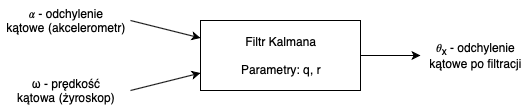
\includegraphics[width=0.75\textwidth]{Rysunki/Rozdzial04/Kalman_idea.png}
    \caption{Zmienne wejściowe oraz wyjściowe dla filtra Kalmana}
    \label{Kalman idea}
\end{figure}

Dane wejściowe podawane są w następujących jednostkach
\begin{itemize}
    \item $\alpha (^o)$
    \item $\omega (^0/s)$
\end{itemize}

Do działania filtru konieczne jest zamodelowanie obiektu w postaci równań stanu. W tym celu zaproponowano równanie opisujące system
$$
    \theta_x(t) = \theta_x(t-1) + (\omega_x(t-1) - \zeta_x)\Delta t
$$
co można rozpisać na następujące równania
\begin{equation}
    \begin{array}{l}
        \theta_x(t) = \theta_x(t-1) - \zeta_x(t-1)\Delta t + \omega\Delta t \\
        \omega_x(t) = \omega - \zeta_x(t-1) \\
        \zeta_x(t) = \zeta_x(t-1)
    \end{array}
    \label{Rownania obiektu}
\end{equation}
gdzie wartości na wyjściu systemu to odpowiednio
\begin{itemize}
    \item $\theta_x$ -- wartość odchylenia kątowego 
    \item $\omega_x$ -- wartość prędkości kątowej 
    \item $\zeta_x$ -- wartość błędu żyroskopu (dryf)
\end{itemize}

Mając równania systemu w takiej postaci, możemy zapisać je w postaci macierzowej, czyli sformułować równania stanu obiektu.
%----------------------------------------------------------------------------------------------------------------
\subsection{Równanie stanu obiektu}
Równanie stanu sformułowane na podstawie równań (\ref{Rownania obiektu})
$$
    x(t) = Ax(t-1) + Bu
$$
gdzie
$$
    \mathbf{A} =
    \left[
    \begin{array}{ccc}
        1 & 0 & -\Delta t \\
        0 & 0 & -1 \\
        0 & 0 & 1
    \end{array}
    \right]
    \quad
    \mathbf{B} = 
    \left[
    \begin{array}{c}
        \Delta t \\
        1 \\
        0
    \end{array}
    \right]
$$
%
Wektor stanu
$$
    \mathbf{x} = 
    \left[
    \begin{array}{c}
        \theta_x \\
        \omega_x \\
        \zeta_x
    \end{array}
    \right]
$$
%
W tym przypadku sterowaniem systemu jest prędkość kątowa odczytana z żyroskopu
$$
    \mathbf{u} = \omega
$$
%
Z racji tego, że na wyjściu systemu istotne dla nas jest aktualne odfiltrowane odchylenie kątowe $\theta_x$ przechowywane w wektorze stanu po aktualizacji, macierz wyjścia przyjmuje postać
$$
    \mathbf{C} = 
    \left[
    \begin{array}{ccc}
        1 & 0 & 0
    \end{array}
    \right]
$$
%
Macierz kowariancji pomiaru, w pierwszej iteracji algorytmu przyjmuje postać macierzy diagonalnej, mającej na swej diagonali wartości wariancji pomiaru
$$
    \mathbf{P} = 
    \left[
    \begin{array}{ccc}
        r & 0 & 0 \\
        0 & r & 0 \\
        0 & 0 & r
    \end{array}
    \right]
$$
%
Macierz kowariancji procesu, w pierwszej iteracji algorytmu przyjmuje postać macierzy diagonalnej, mającej na swej diagonali wartości wariancji procesu
$$
    \mathbf{Q} = 
    \left[
    \begin{array}{ccc}
        q & 0 & 0 \\
        0 & q & 0 \\
        0 & 0 & q
    \end{array}
    \right]
$$
%
Macierz szumu akcelerometru jest jedno wymiarowa i przyjmuje wartość wariancji pomiaru
$$
    \mathbf{R} = r
$$

%----------------------------------------------------------------------------------------------------------------
\subsection{Równania filtru Kalmana}

Faza predykcji
\begin{enumerate}
    \item prognoza stanu: $$x(t) = Ax(t-1) + B \omega$$
    \item prognoza błędu kowariancji: $$P(t) = AP(t-1)A^T+Q$$
\end{enumerate}
%
Faza korekcji
\begin{enumerate}
    \item wzmocnienie filtra Kalmana: $$K(t) = P(t)H^TH(HP(t)H^T+R)^{-1}$$
    \item aktualizacja estymacji w oparciu o rzeczywisty pomiar: $$x(t) = x(t) + K(t)(\alpha - Hx(t))$$
    \item aktualizacja błędu kowariancji: $$P(t) = (1 - K(t)H)P(t)$$
\end{enumerate}

W każdej iteracji działania algorytmu, aktualny kąt wychylenia $\theta_x$ znajduje się w zaktualizowanym wektorze stanu. Jest to wartość wyjściowa filtra pozbawiona zakłóceń.

%----------------------------------------------------------------------------------------------------------------
\section{Filtr Madgwicka}

W 2010 roku S.O Madgwick opublikował raport \cite{Madgwick2010AnEO} dotyczący opracowanego przez siebie algorytmu do uzyskiwania orientacji w przestrzeni czujników MARG. Przewagą jaką ma owy filtr nad innymi znanymi filtrami jest to, że nie wymaga on kalibracji magnetometru. Algorytm samodzielnie radzi sobie z odkształceniami ,,hard iron'' oraz ,,soft iron''. Drugą dużą zaletą jest odporność na tzw. efekt ,,gimbal lock'', który jest poważną wadą przy opisie orientacji za pomocą kątów RPY oraz Eulera. Objawia się on maksymalnym zakresem dla kąta Pitch wynoszącym $<-90^o, 90^o>$, co wynika z maksymalnej oraz minimalnej wartości jaką przyjmuje funkcja arcus sinus.

Inne zalety jakie w swoim raporcie wymienia autor to m.in niski koszt obliczeniowy, dzięki czemu algorytm z powodzeniem można implementować na słabszych mikroprocesorach oraz wysoka skuteczność przy niskich częstotliwościach próbkowania czujników, np. 10Hz.

\begin{figure}[h!]
    \centering
    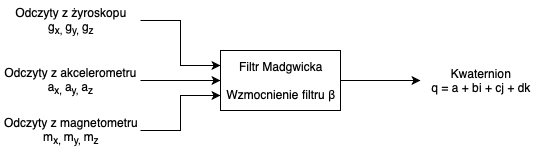
\includegraphics[width=0.75\textwidth]{Rysunki/Rozdzial04/Madgwick_idea.png}
    \caption{Zmienne wejściowe oraz wyjściowe dla filtra Madgwicka}
    \label{Madgwick idea}
\end{figure}

Dane wejściowe podawane są w następujących jednostkach
\begin{itemize}
    \item $g_x, g_y, g_z (rad/s)$
    \item $a_x, a_y, a_z (g)$
    \item $m_x, m_y, m_z (\mu T)$
\end{itemize}

Do matematycznego opisu orientacji w przestrzeni algorytm wykorzystuje kwaterniony, które z powodzeniem można przeliczyć na kąty RPY
$$
    \begin{array}{l}
        Roll = arctan\left(\frac{2(ab + cd)}{1 - 2(b^2 + c^2)}\right) \\ \\
        Pitch = -arcsin(2(ac + db)) \\ \\
        Yaw = arctan\left(\frac{2(ad + bc)}{1 - 2(c^2 + d^2)}\right) 
    \end{array}
$$

%----------------------------------------------------------------------------------------------------------------
\subsection{Poszczególne etapy działania algorytmu}

\begin{enumerate}
    \item Wyznaczenie szybkości zmiany orientacji kwaternionu na podstawie wektora prędkości kątowych
    $$
        _E^S \Dot{q}_{\omega,t} = \frac{1}{2} \ _E^S \hat{q}_{est,t-1} \tens \ \omega
    $$
    gdzie \\
    $ \tens \ $ -- iloczyn tensorowy \\
    $ _E^S \hat{q}_{est,t-1} $ -- znormalizowany kwaternion z poprzedniej iteracji\\
    $ \omega $ -- wektor prędkości kątowych
    \item Wyznaczenie kierunku referencyjnego pola magnetycznego oraz współczynnika korygującego zaburzenia pola magnetycznego
    $$
        \begin{array}{cc}
            ^E \hat{h_t} = _E^S \hat{q} \tens \ \hat{m_t} \tens \ \ _E^S \hat{q}^{*} = [0 \quad h_x \quad h_y \quad h_z] \\ \\
            ^E \hat{b_t} = [0 \quad \sqrt{h_x^2 + h_y^2} \quad 0 \quad h_z]
        \end{array}
    $$
    gdzie \\
    $ \hat{m_t} $ -- znormalizowany wektor pomiarów z magnetometru\\
    $ _E^S \hat{q}^{*} = _S^E \hat{q} $ -- sprzężenie kwaternionu orientacji
    \item Znalezienie minimum lokalnego funkcji celu
    $$
        f(_E^S \hat{q}, \hat{d}, \hat{s}) = _E^S \hat{q}^{*} \tens \ \hat{d} \tens \ \ _E^S \hat{q} - \hat{s}
    $$
    metodą gradientu prostego w wyniku, które otrzymujemy błąd zmiany orientacji w danym zakresie czasu
    $$
        _E^S \Dot{\hat{q}}_{s,t}
    $$
    który pozwala na wyznaczenie estymaty wartości szybkości zmiany orientacji kwaternionu
    $$
        _E^S \Dot{q}_{est,t} = _E^S \Dot{q}_{\omega,t} - \beta _E^S \Dot{\hat{q}}_{s,t}
    $$
    \item Całkując szybkość zmiany orientacji kwaternionu po czasie otrzymujemy aktualną orientację kwaternionu 
    $$
        _E^S q_{est,t} = _E^S q_{est,t-1} + _E^S \Dot{q}_{est,t} \Delta t
    $$
    którą możemy wykorzystać do obliczenia kątów RPY, lub pozostawić w postaci kwaternionu jeśli bazujemy na takiej metodzie określania orientacji w przestrzeni, jednak jest ona dosyć nieintuicyjna i mało czytelna na pierwszy rzut oka. 
    
\end{enumerate}

%----------------------------------------------------------------------------------------------------------------
\section{Testy symulacyjne}

Testy opisanych wcześniej trzech algorytmów przeprowadzone zostały w środowisku \texttt{Matlab Simulink}, z wykorzystaniem danych pochodzących z rzeczywistego modułu MARG MPU9250. Dane zostały wprowadzone w następujących jednostkach
\begin{itemize}
    \item Żyroskop -- prędkość kątowa ($^o/s$) 
    \item Akcelerometr -- przyspieszenie ($g$)
    \item Magnetometr -- indukcja pola magnetycznego ($\mu T$) 
\end{itemize}

Przed zapisaniem danych czujnik został skalibrowany, o czym więcej w kolejnym rozdziale \ref{chap:budowa} dotyczącym budowy robota balansującego. Wczytane dane zaprezentowane zostały na rysunku \ref{MARG sygnaly}
\begin{figure}[h!]
    \centering
    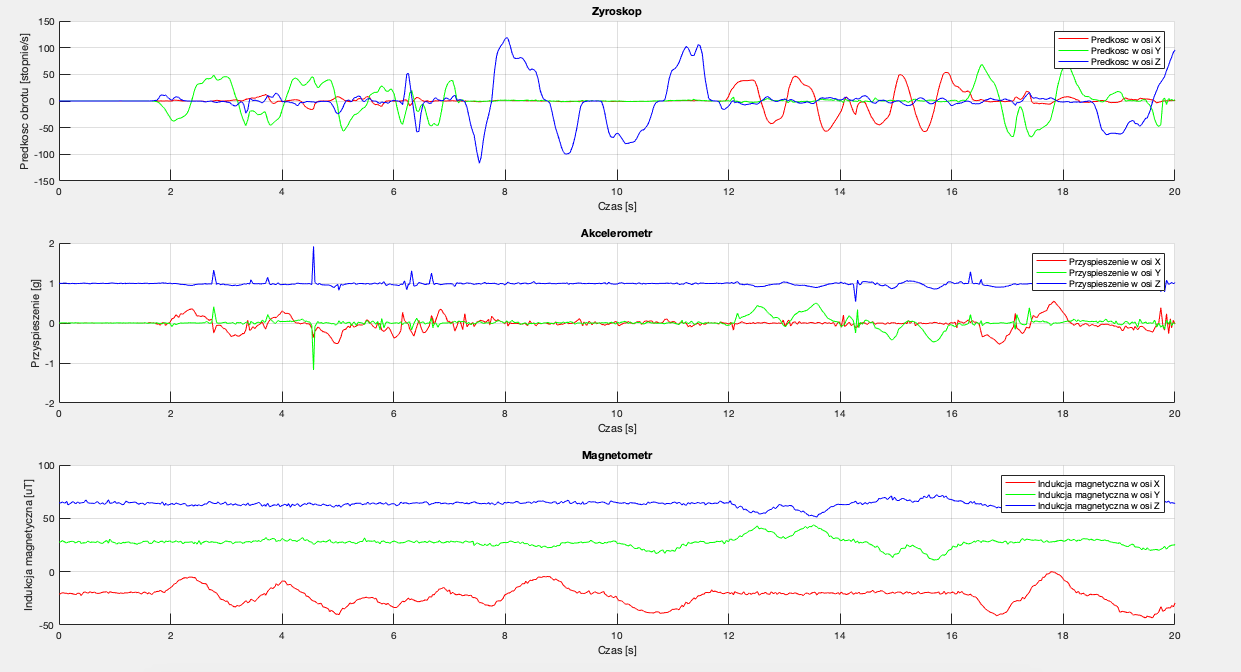
\includegraphics[width=1\textwidth]{Rysunki/Rozdzial04/MARG_sygnaly.png}
    \caption{Sygnały z modułu wykorzystane podczas symulacji}
    \label{MARG sygnaly}
\end{figure}

\newpage
%----------------------------------------------------------------------------------------------------------------
\subsection{Filtr komplementarny}

Do implementacji filtra komplementarnego, wykorzystano bloczki \texttt{Transfer Fcn}, do których zostały wprowadzone odpowiednie transmitancje, oraz stała czasowa wczytywana ze skryptu.
\begin{figure}[h!]
    \centering
    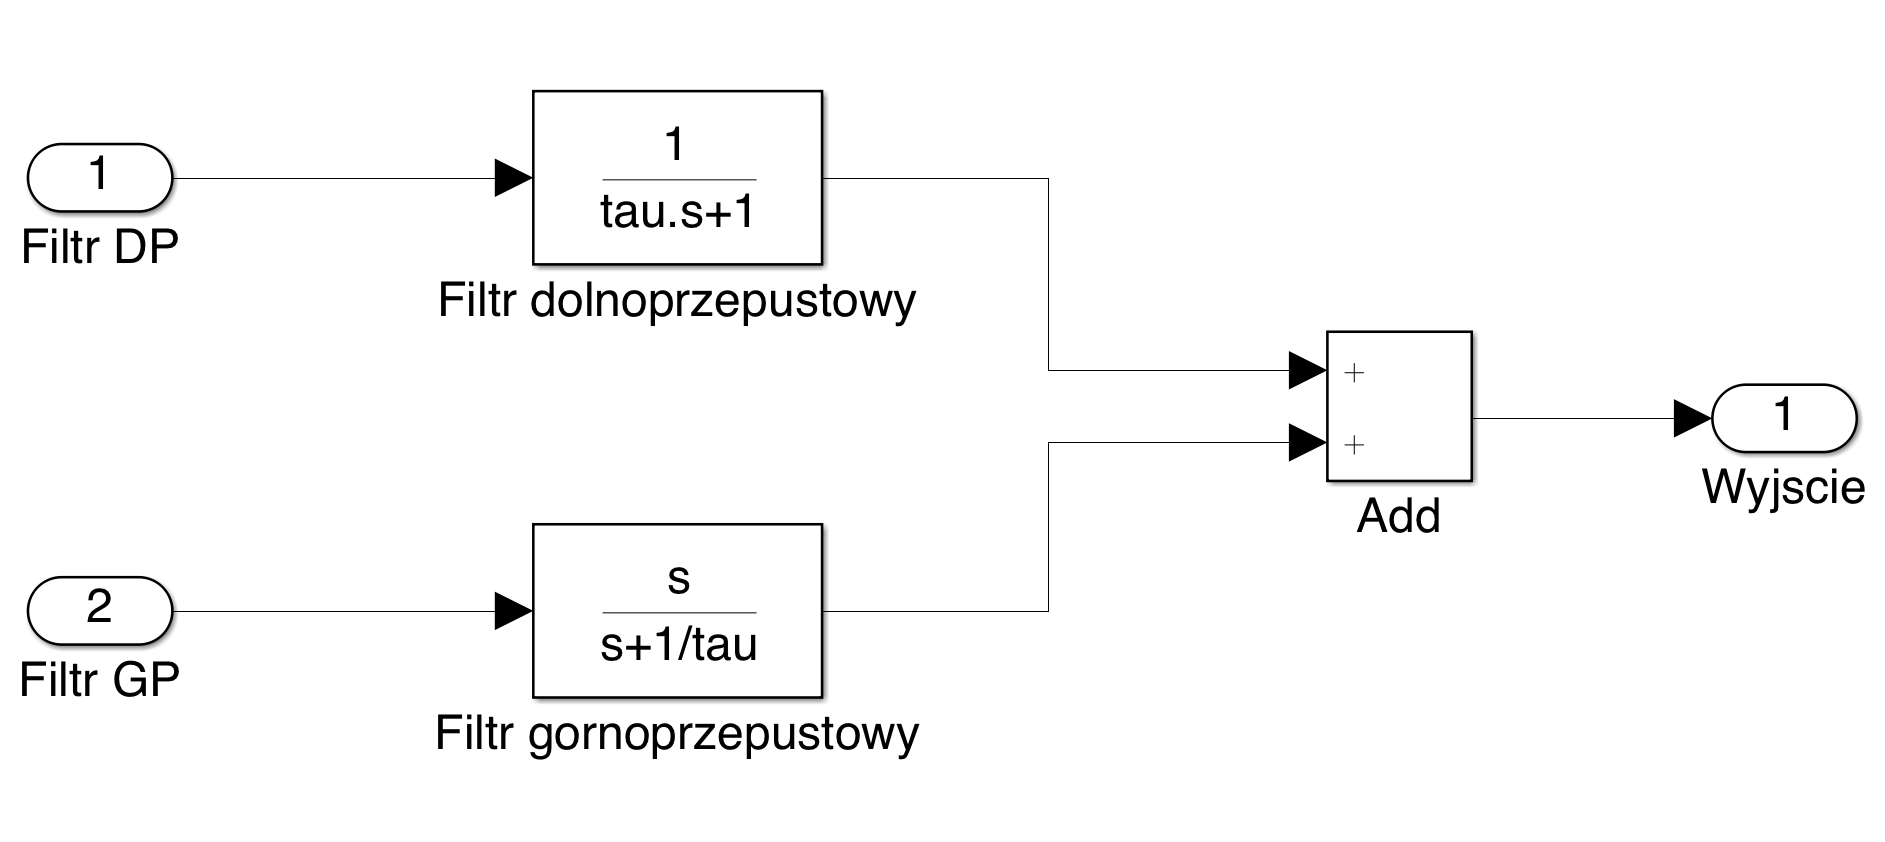
\includegraphics[width=0.75\textwidth]{Rysunki/Rozdzial04/Filtr_komplementarny_implementacja.png}
    \caption{Implementacja filtra komplementarnego}
    \label{Komplementarny implementacja}
\end{figure}

Filtr komplementarny wykorzystano do uzyskania rotacji w trzech osiach. Rotację w osiach X i Y uzyskano na podstawie pomiarów z akcelerometru i żyroskopu, a rotację w okół osi Z na podstawie pomiarów z magnetometru i żyroskopu

\newpage
\begin{figure}[h!]
    \centering
    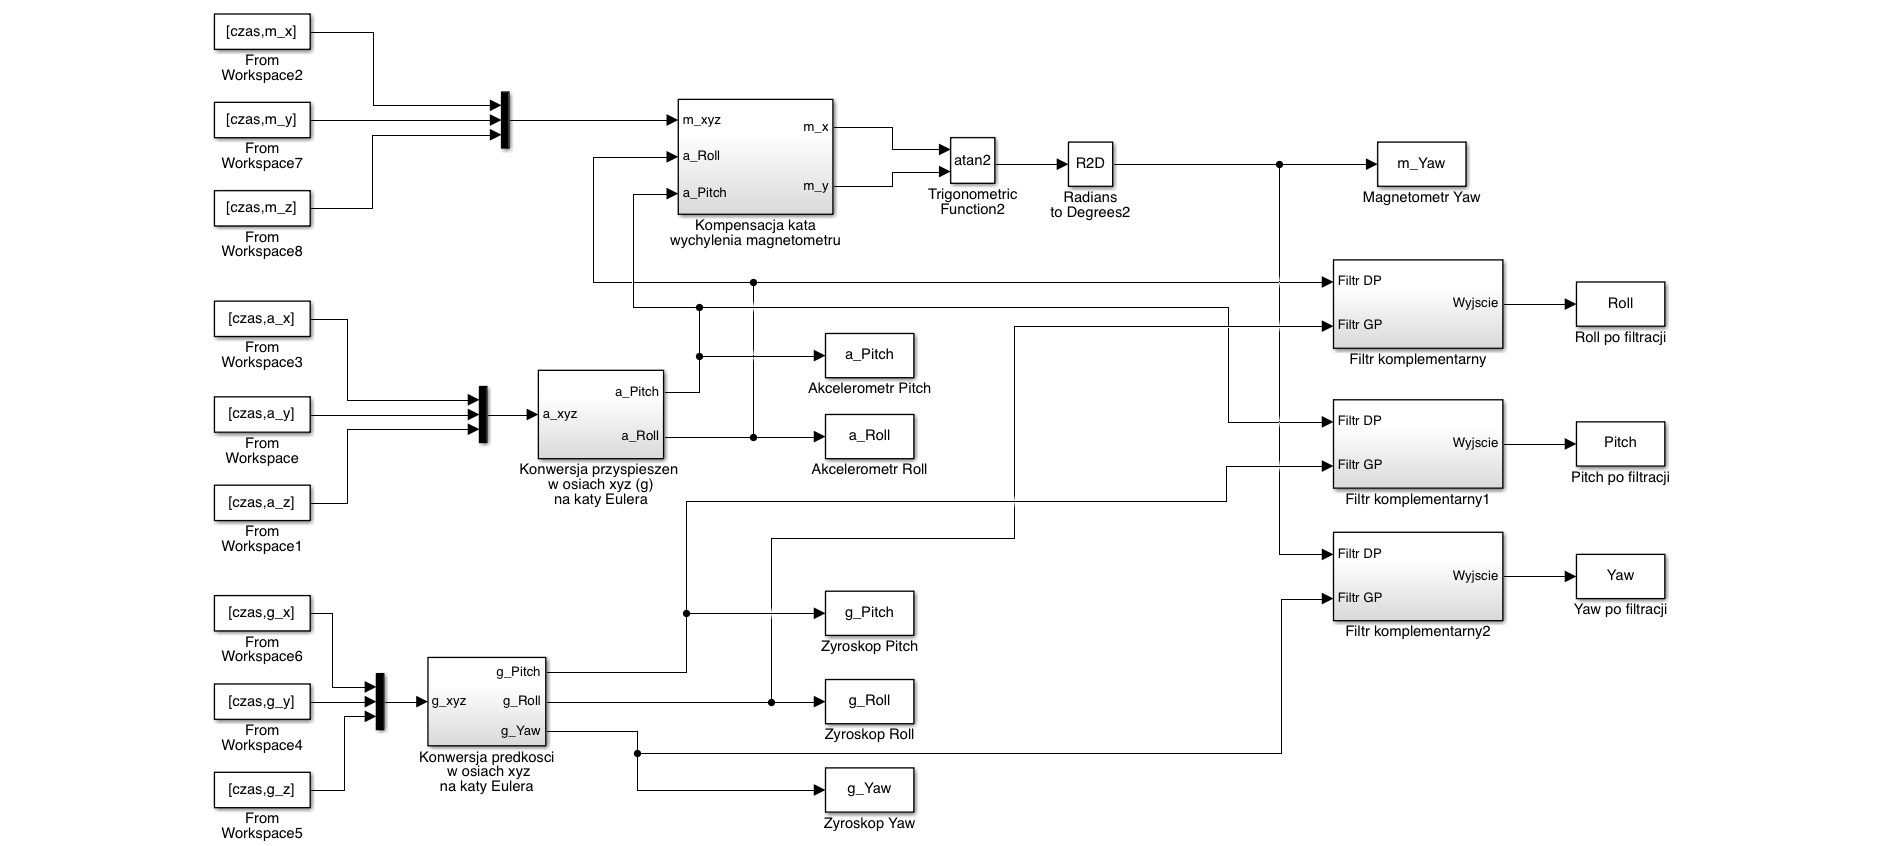
\includegraphics[width=1\textwidth]{Rysunki/Rozdzial04/Filtr_komplementarny_struktura_png.png}
    \caption{Wykorzystanie filtra komplementarnego dla sygnałów z akcelerometru, żyroskopu i magnetometru}
    \label{Komplementarny struktura}
\end{figure}

 Na rysunku \ref{Komplementarny przed} widać, że akcelerometr i magnetometr obarczony jest szybkozmiennymi zakłóceniami, a żyroskop wolnozmiennymi.
\begin{figure}[h!]
    \centering
    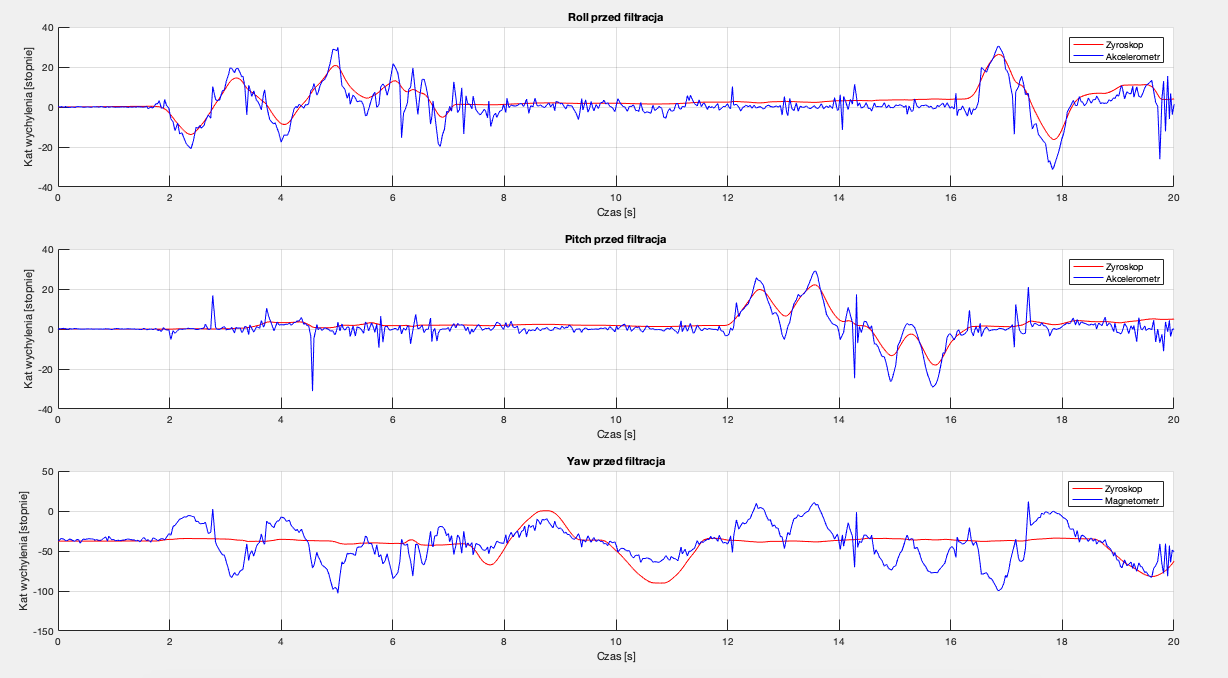
\includegraphics[width=1\textwidth]{Rysunki/Rozdzial04/Filtr_komplementarny_przed.png}
    \caption{Sygnały wejściowe dla filtra komplementarnego}
    \label{Komplementarny przed}
\end{figure}

W trakcie testowania algorytmu zdecydowano się dobrać trzy wartości stałej czasowej
$$
    \begin{array}{ccc}
        \tau_1 = 1 & \tau_2 = 0.01 & \tau_3 = 0.0001
    \end{array}
$$
które odpowiadają odpowiednio parametrowi filtra przy czasie próbkowania $\Delta t = 0.01s$
$$
    \begin{array}{ccc}
        \beta_1 \approx 0.99 & \beta_2 = 0.5 & \beta_3 \approx 0.009
    \end{array}
$$

\begin{figure}[h!]
    \centering
    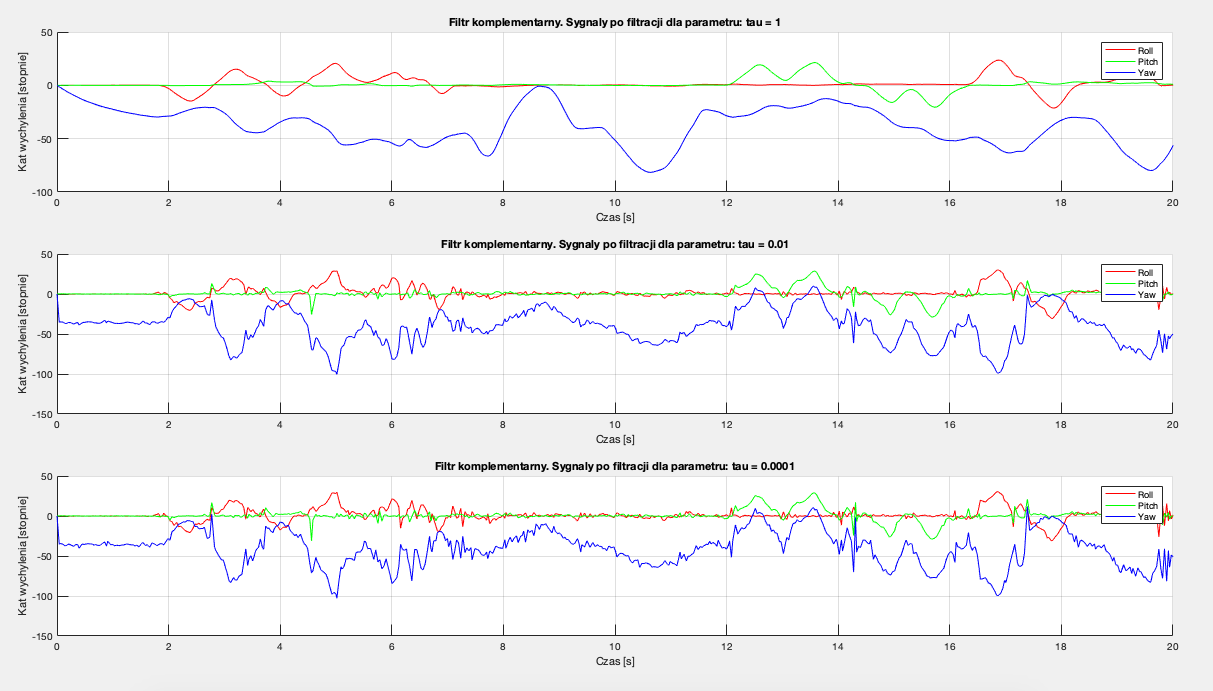
\includegraphics[width=1\textwidth]{Rysunki/Rozdzial04/Filtr_komplementarny_po.png}
    \caption{Sygnały wyjściowe dla filtra komplementarnego}
    \label{Komplementarny po}
\end{figure}

Stała czasowa decyduje o tym, jaką część z ostatecznej wartości na wyjściu filtra stanowi pomiar z akcelerometru lub magnetometru, a jaką pomiar z żyroskopu. Stąd wywnioskowano, że im większa stała czasowa tym większy udział w ostatecznym wyniku ma pomiar z żyroskopu (mniej widocznych zakłóceń szybkozmiennych).
%----------------------------------------------------------------------------------------------------------------
\subsection{Filtr Kalmana}

Sygnałami wejściowymi dla filtra Kalmana są obarczone zakłóceniami szybkozmiennymi kąty obliczone na podstawie odczytów z akcelerometru oraz prędkości kątowe odczytane za pomocą żyroskopu, rysunek \ref{Kalman przed}

\begin{figure}[h!]
    \centering
    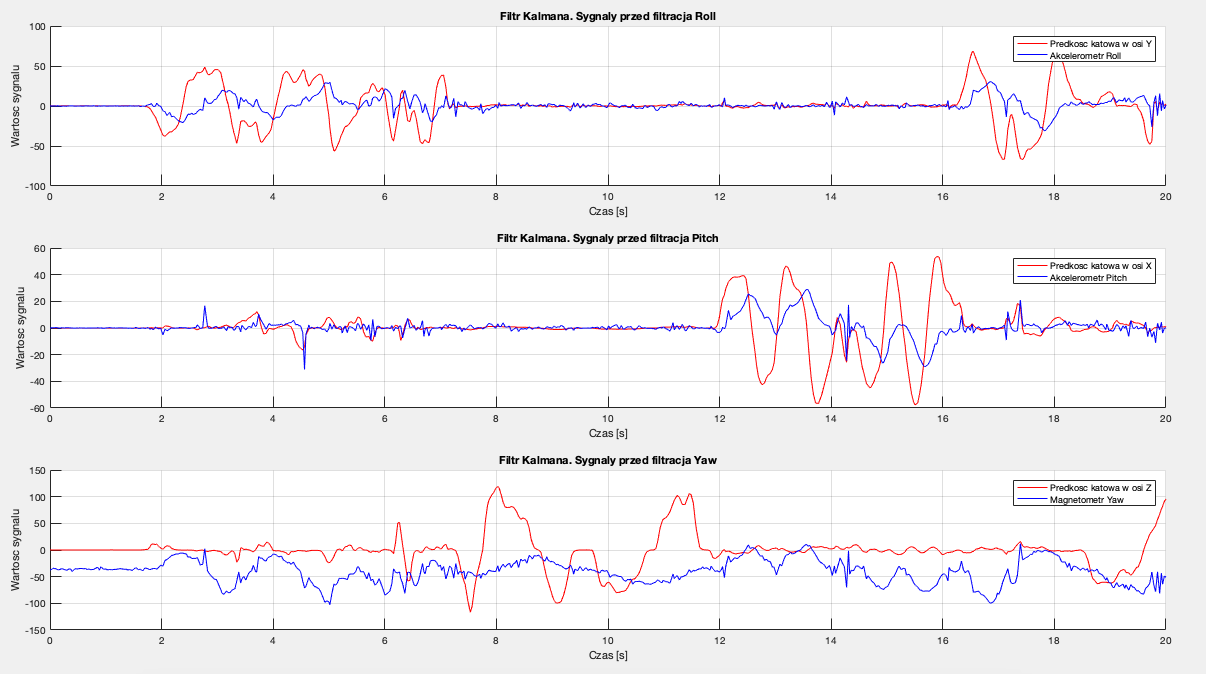
\includegraphics[width=1\textwidth]{Rysunki/Rozdzial04/Filtr_Kalmana_przed.png}
    \caption{Sygnały wejściowe dla filtra Kalmana}
    \label{Kalman przed}
\end{figure}

W celach eksperymentalnych spróbowano zastosować kąty obliczone na podstawie odczytów z magnetometru zamiast akcelerometru do wyznaczenia obrotu wokół osi Z. Z powodzeniem uzyskano wyniki zbliżone do filtra komplementarnego. Dodatkowo przetestowano algorytm dla trzech par parametrów
$$
    \begin{array}{ll}
        r_1 = 1000 & q_1 = 10000 \\
        r_2 = 1 & q_2 = 1 \\
        r_3 = 0.0001 & q_3 = 10 
    \end{array}
$$
\begin{figure}[h!]
    \centering
    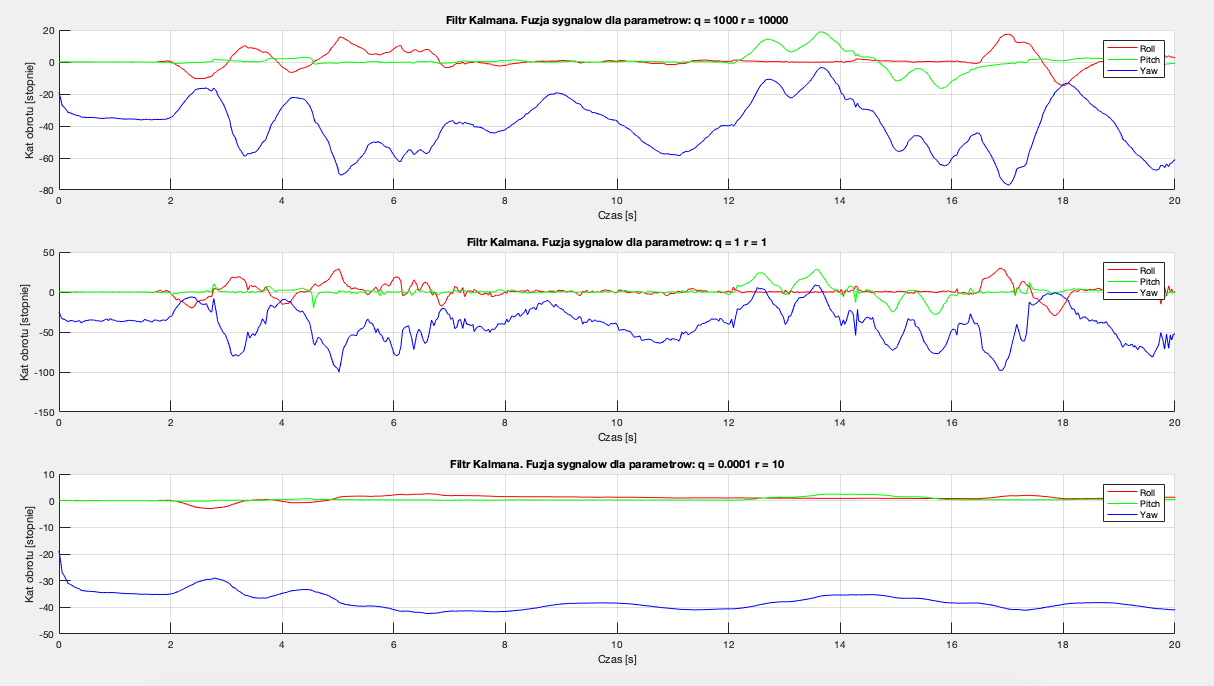
\includegraphics[width=1\textwidth]{Rysunki/Rozdzial04/Filtr_Kalmana_po.png}
    \caption{Sygnały wyjściowe dla filtra Kalmana}
    \label{Kalman po}
\end{figure}

%----------------------------------------------------------------------------------------------------------------
\subsection{Filtr Madgwicka}

\begin{figure}[h!]
    \centering
    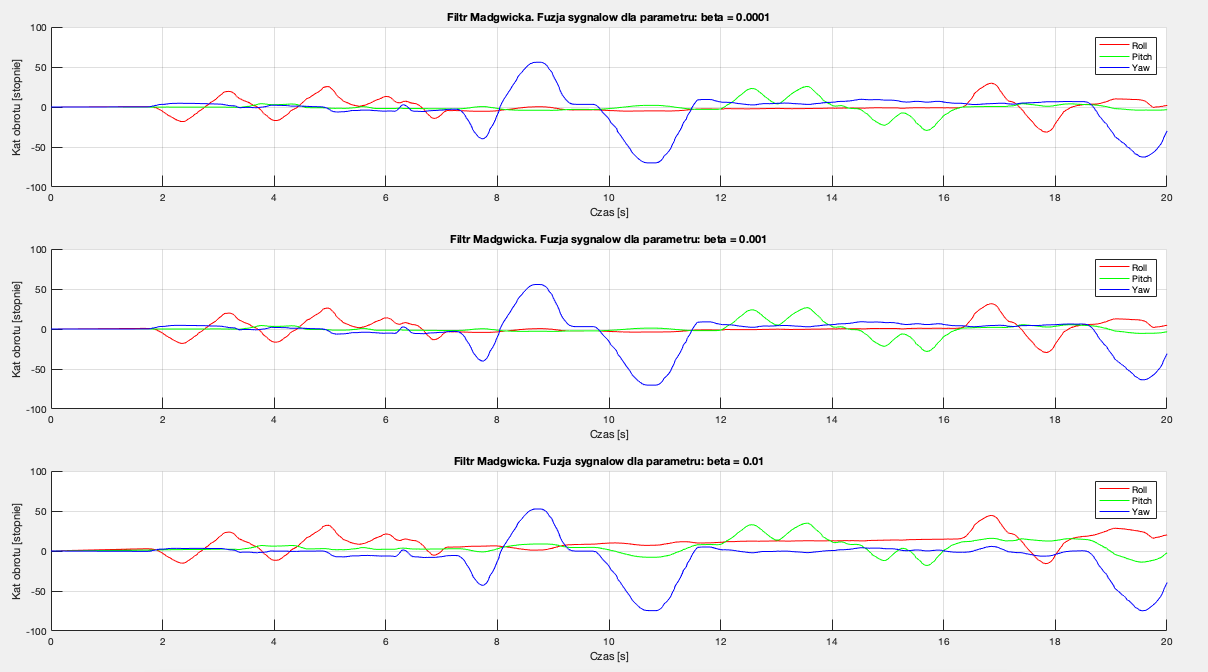
\includegraphics[width=1\textwidth]{Rysunki/Rozdzial04/Filtr_Madgwicka_po.png}
    \caption{Sygnały wyjściowe dla filtra Madgwicka}
    \label{Madgwick po}
\end{figure}

%----------------------------------------------------------------------------------------------------------------
\subsection{Porównanie filtrów}

W teście wykorzystano następujące parametry filtrów
\begin{table}[h!]
    \centering
    \begin{tabular}{|c|c|c|}
        \hline
        F.komplementarny & F.Kalmana & F.Madgwicka \\
        \hline
        $\tau = 0.1$ & $r = 10000$, $q = 1000$ & $\beta = 0.001$ \\
        \hline
    \end{tabular}
    
     \caption{Parametry filtrów przyjęte podczas porównania}
\end{table}

Dla kątów Roll oraz Pitch algorytmy działają podobnie, jednak dla kąta Yaw widać znaczną przewagę filtra Madgwicka, który zdecydowanie lepiej poradził sobie z zakłóceniami szybkozmiennymi pochodzącymi od magnetometru. Wyraźnie widoczne jest to między sekundą 0-7 oraz 12-17 na wykresie \ref{Porownanie}. Kiedy chciano poprawić działanie filtra komplementarnego i Kalmana dla kąta Yaw, tak aby osiągnąć wynik zbliżony do tego dla filtra Madgwicka, nie przyniosło to zadowalających rezultatów. Owszem zakłócenia zostały zniwelowane, ale sygnały zaczęły znacząco odbiegać od rzeczywistości. 

\begin{figure}[h!]
    \centering
    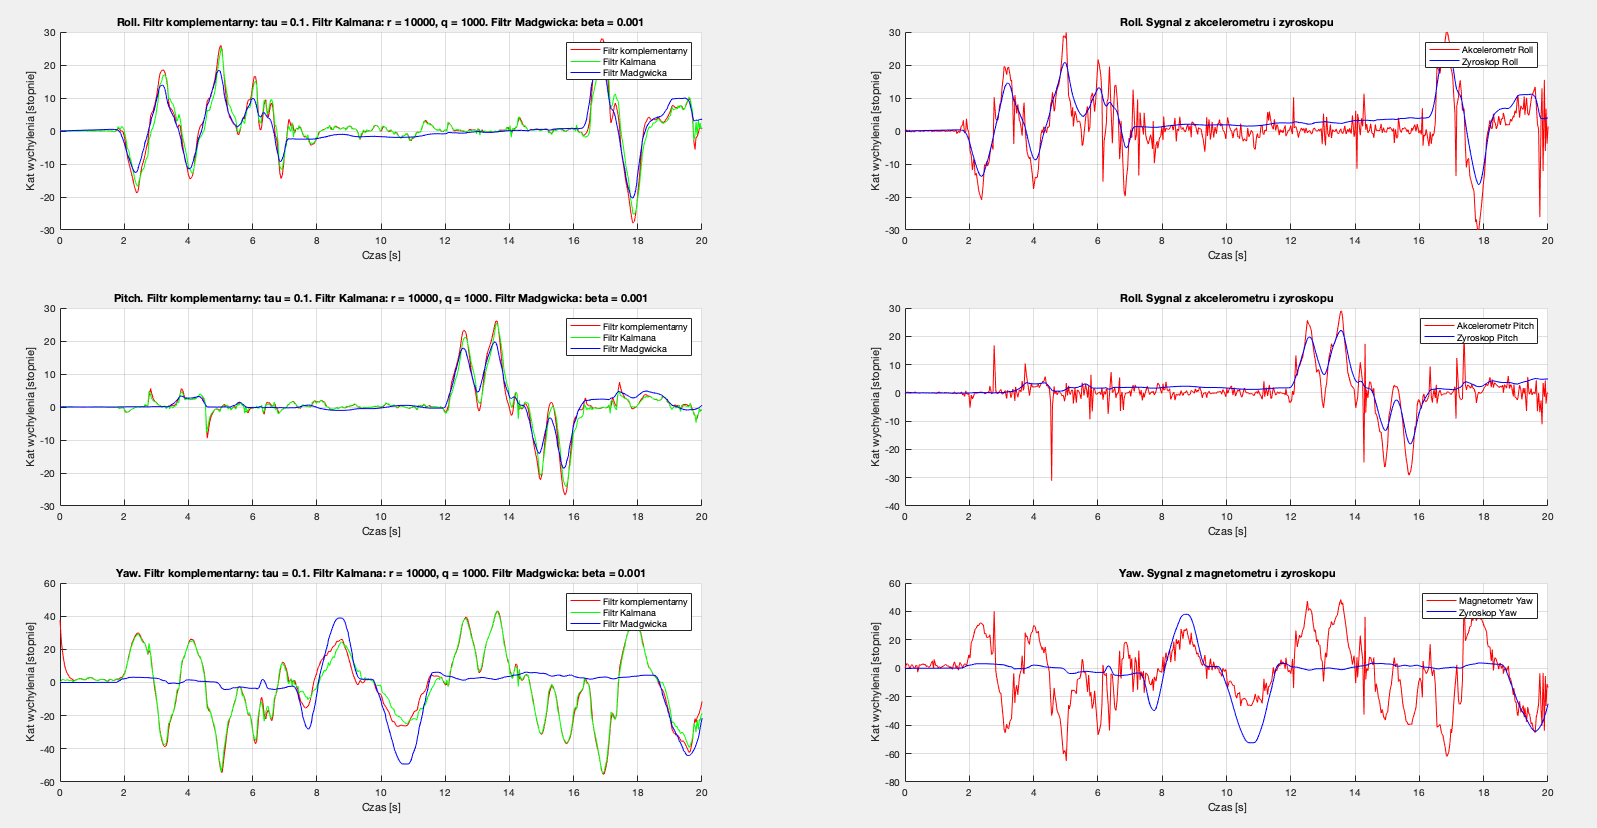
\includegraphics[width=1\textwidth]{Rysunki/Rozdzial04/Porownanie.png}
    \caption{Wykresy zbiorcze dla wszystkich filtrów}
    \label{Porownanie}
\end{figure}

Warto też dodać, że wartość początkowa kąta obliczanego na podstawie odczytów z żyroskopu wynosi 0. Tak aby porównanie działania filtrów było miarodajne, należy przesunąć kąt obliczany na podstawie odczytów z żyroskopu o pewną wartość względem pomiarów obliczanych na podstawie odczytów z magnetometru, tak aby w chwili $t = 0$ oba wykresy miały tą samą wartość.